\section{Exercise 01}
\subsection{}

\begin{frame}
\frametitleTC{Direct synthesis for set point tracking}
\framesubtitleTC{Some examples}
\myPause
 \begin{itemize}[<+-| alert@+>]
 \item Example 1 (OK):
       \begin{displaymath}
        \begin{array}{lcl}
         P(z)              = \frac{(z-0.5)}{(z-0.4)^2},\,
         G_{yw}^{\circ}(z) = \frac{0.2}{z-0.8} &
         \Rightarrow &
         C(z)              = \frac{0.2(z-0.4)^2}{(z-1)(z-0.5)}.
        \end{array}
       \end{displaymath}
 \item Example 2 (\red{NO}, process pole outside the circle $\Rightarrow$ unstable hidden part):
       \begin{displaymath}
        \begin{array}{lcl}
         P(z)              = \frac{1}{\red{z-2}},\,
         G_{yw}^{\circ}(z) = \frac{0.2}{z-0.8} &
         \Rightarrow &
         C(z)              = \frac{0.2\red{(z-2)}}{z-1}.
        \end{array}
       \end{displaymath}
 \item Example 3 (\red{NO}, infeasible relative degree):
       \begin{displaymath}
        \begin{array}{lcl}
         P(z)              = \frac{1}{(z-0.4)^2},\,
         G_{yw}^{\circ}(z) = \frac{0.2}{z-0.8} &
         \Rightarrow &
         C(z)              = \frac{0.2(z-0.4)^{\textcolor{red}{2}}}{z-1}.
        \end{array}
       \end{displaymath}
 \item Try one/two cases of your own, verify that everything is clear,\\
       ask questions if necessary.
 \end{itemize}
\end{frame}

\begin{frame}
\frametitleTC{Direct synthesis for set point tracking}
\framesubtitleTC{Dealing with the limitations}
\myPause
 \begin{itemize}[<+-| alert@+>]
 \item If the process has poles on or outside the circle, we must preserve them in the desired loop transfer
       function
       \begin{displaymath}
        L^{\circ}(z) = \frac{G_{yw}^{\circ}(z)}{1-G_{yw}^{\circ}(z)}
       \end{displaymath}
       so as to not have $C(z)$ cancel them and generate an unstable hidden part.
 \item If the process has zeroes on or outside the circle, we must include them in $G_{yw}^{\circ}(z)$\\
       -- hence in $L^{\circ}(z)$ -- so that $C(z)$ does not cancel them either; this may\\
       require to also add poles to have at least as many as there are zeroes.
 \item If the relative degree of $G_{yw}^{\circ}(z)$ is infeasible, we need to add ``fast''\\
       (near to the origin) poles and/or delay terms.
 \item\vfill Let us clarify with a few simulation examples. 
 \end{itemize}
\end{frame}


\begin{frame}[fragile]
\frametitleTC{Direct synthesis for set point tracking}
\framesubtitleTC{Dealing with the limitations -- Scilab script (1/3, copy{\&}paste to try at home)}
{\tiny
\def\baselinestretch{0.3}
\begin{verbatim}
// Direct synthesis examples -- set point tracking
clear; clc; z = %z;
// Reference and time vectors
w  = ones(1,30); 
k  = 0:length(w)-1;
// Process 1, asymptotically stable, no zeroes
P1 = syslin('d',2/(z-0.5)^2);
// Infeasible relative degree
To = syslin('d',0.2/(z-0.8));
R  = 1/P1*To/(1-To); disp(R); y1 = dsimul(tf2ss(To),w);
// Adding a fast pole for a realisable R
To = syslin('d',0.16/(z-0.8)/(z-0.2));
R  = 1/P1*To/(1-To); disp(R); y2 = dsimul(tf2ss(To),w);
// Adding a faster pole
To = syslin('d',0.19/(z-0.8)/(z-0.05));
R  = 1/P1*To/(1-To); disp(R); y3 = dsimul(tf2ss(To),w);
// Adding a one-step delay
To = syslin('d',0.2/(z-0.8)/z);
R  = 1/P1*To/(1-To); disp(R); y4 = dsimul(tf2ss(To),w);
// Using two poles, both faster than the design one
p1 = 0.75;
p2 = 0.45;
To = syslin('d',(1-p1)*(1-p2)/(z-p1)/(z-p2));
R  = 1/P1*To/(1-To); disp(R); y5 = dsimul(tf2ss(To),w);
\end{verbatim}
}
\end{frame}

\begin{frame}[fragile]
\frametitleTC{Direct synthesis for set point tracking}
\framesubtitleTC{Dealing with the limitations -- Scilab script (2/3)}
{\tiny
\def\baselinestretch{0.3}
\begin{verbatim}
// Process 2, asymptotically stable,, 1 zero outside the circle
P2 = syslin('d',(z-2)/(z-0.5)^2);
// Infeasible To
To = syslin('d',0.2/(z-0.8));
R  = 1/P2*To/(1-To); disp(R); y6 = dsimul(tf2ss(To),w);
// Adding the required zero to To
To = syslin('d',-0.18*(z-2)/(z-0.8)/(z-0.1));
R  = 1/P2*To/(1-To); disp(R); y7 = dsimul(tf2ss(To),w);
// Improving by acting on the To poles
p1 = 0.78;
p2 = 0.02;
To = syslin('d',-(1-p1)*(1-p2)*(z-2)/(z-p1)/(z-p2));
R  = 1/P2*To/(1-To); disp(R);
y8 = dsimul(tf2ss(To),w);
\end{verbatim}
}
\end{frame}

\begin{frame}[fragile]
\frametitleTC{Direct synthesis for set point tracking}
\framesubtitleTC{Dealing with the limitations -- Scilab script (3/3)}
{\tiny
\def\baselinestretch{0.3}
\begin{verbatim}
// Plot the results for process 1
h               = scf(0); clf;
h.figure_size   = [500,500];
title("${\Large \text{Cases 1--5}$");
xlabel("k");
plot(k,y1,'r',k,y1,'r.');
plot(k,y2,'b',k,y2,'b.');
plot(k,y3,'m',k,y3,'m.');
plot(k,y4,'g',k,y4,'g.');
plot(k,y5,'k',k,y5,'k.');
ax              = gca();
ax.data_bounds  = [0,0;max(k),1.1];
ax.tight_limits = "on";
// Plot the results for process 2
h               = scf(1); clf;
h.figure_size   = [500,500];
title("${\Large \text{Cases 6--8}$");
xlabel("k");
plot(k,y6,'r',k,y6,'r.');
plot(k,y7,'b',k,y7,'b.');
plot(k,y8,'k',k,y8,'k.');
ax              = gca();
ax.data_bounds  = [0,-0.3;max(k),1.1];
ax.tight_limits = "on";
\end{verbatim}
}
\end{frame}

\begin{frame}
\frametitleTC{Synthesis for set point tracking}
\framesubtitleTC{Dealing with the limitations -- summary}
\myPause
\begin{center}
 {\scriptsize
 \begin{tabular}{llll}
  \hline
Case & Process                   & Requirement                                                           & Controller  \\
\hline\hline
1& $P_1(z)=\frac{2}{(z-0.5)^2}$  & $G_{yw,11}^{\circ}(z)=\frac{0.2}{z-0.8}$                              & Infeasible  \\
2&                               & $G_{yw,12}^{\circ}(z)=\frac{0.16}{(z-0.8)(z-0.2)}$                    & $C_{12}(z)$ \\
3&                               & $G_{yw,13}^{\circ}(z)=\frac{0.19}{(z-0.8)(z-0.05)}$                   & $C_{13}(z)$ \\
4&                               & $G_{yw,14}^{\circ}(z)=\frac{0.2}{z(z-0.8)}$                           & $C_{14}(z)$ \\
5&                               & $G_{yw,15}^{\circ}(z)=\frac{(1-0.75)(1-0.45)}{(z-0.75)(z-0.45)}$      & $C_{15}(z)$ \\
\hline
6& $P_2(z)=\frac{z-2}{(z-0.5)^2}$& $G_{yw,21}^{\circ}(z)=\frac{0.2}{z-0.8}$                              & Infeasible  \\
7&                               & $G_{yw,22}^{\circ}(z)=-\frac{0.18(z-2)}{(z-0.8)(z-0.1)}$              & $C_{22}(z)$ \\
8&                               & $G_{yw,23}^{\circ}(z)=-\frac{(1-0.78)(1-0.02)(z-2)}{(z-0.78)(z-0.02)}$& $C_{23}(z)$ \\
  \hline
 \end{tabular}
 }
\end{center}
\end{frame}

\begin{frame}
\frametitleTC{Synthesis for set point tracking}
\framesubtitleTC{Dealing with the limitations -- results}
\myPause
\begin{center}
 {\scriptsize
 \begin{tabular}{ll}
  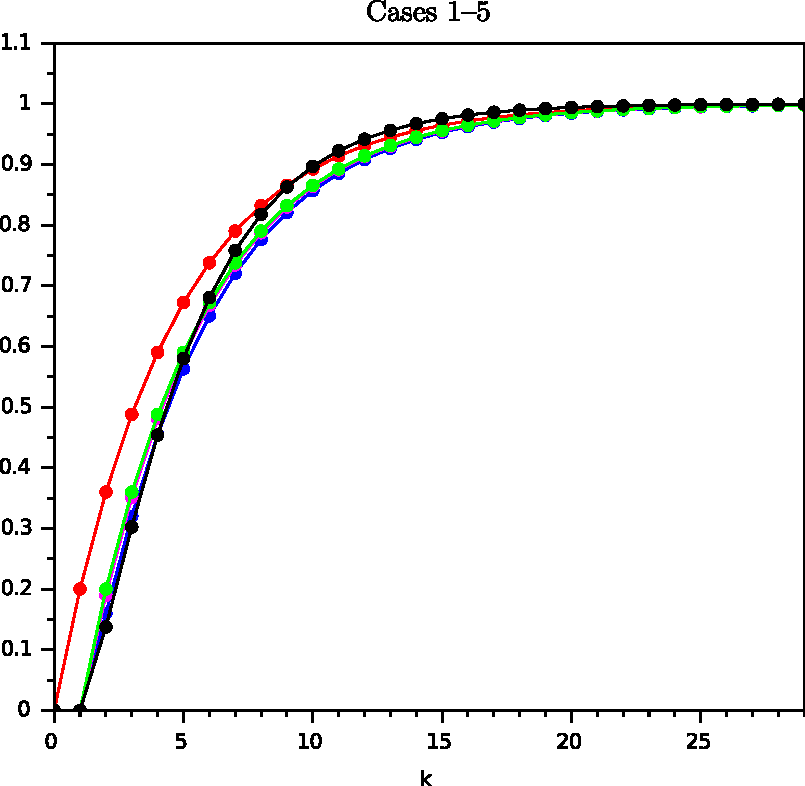
\includegraphics[width=0.35\textwidth]{./Unit-05/img/PS02-ex01-res-1to5.pdf} &
  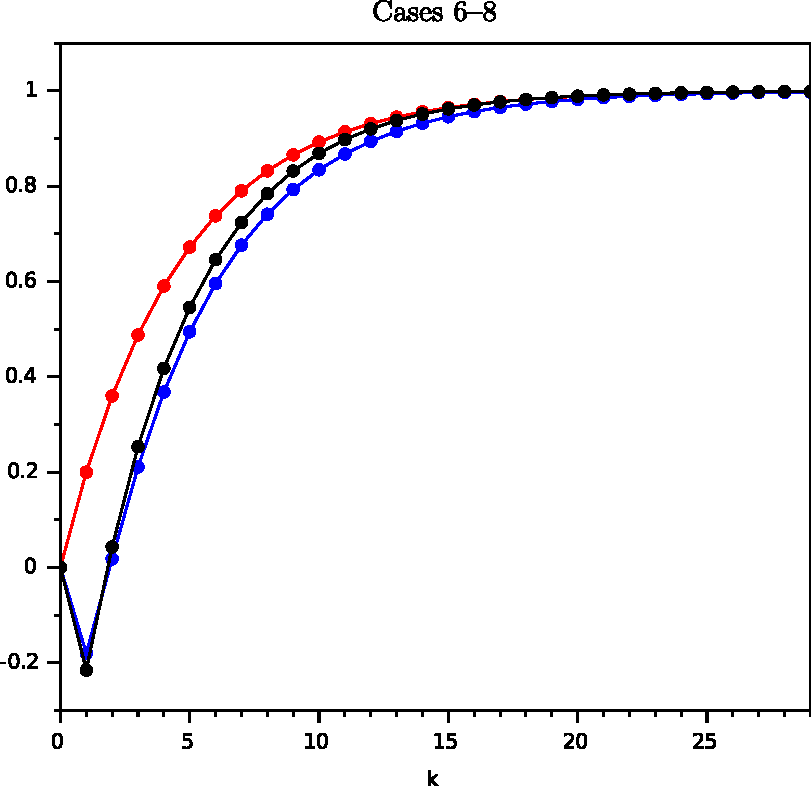
\includegraphics[width=0.35\textwidth]{./Unit-05/img/PS02-ex01-res-6to8.pdf}      \\
   \red{$P_1,G_{yw,11}^{\circ}\Rightarrow$ infeasible} &  \red{$P_2,G_{yw,21}^{\circ}\Rightarrow$ infeasible} \\
  \blue{$P_1,G_{yw,12}^{\circ}\Rightarrow$ $C_{12}$}   & \blue{$P_2,G_{yw,22}^{\circ}\Rightarrow$ $C_{22}$}   \\
   \mgt{$P_1,G_{yw,13}^{\circ}\Rightarrow$ $C_{13}$}   &       $P_2,G_{yw,23}^{\circ}\Rightarrow$ $C_{23}$    \\
   \grn{$P_1,G_{yw,14}^{\circ}\Rightarrow$ $C_{14}$}   \\
        $P_1,G_{yw,15}^{\circ}\Rightarrow$ $C_{15}$    \\
 \end{tabular}
 }
\end{center}
\end{frame}


\begin{frame}
\frametitleTC{Synthesis for set point tracking}
\framesubtitleTC{Summary}
\myPause
 \begin{itemize}[<+-| alert@+>]
 \item The technique is powerful, however there are \TC{objective} limits.
 \item In many of the cases seen the controller has one or two zeroes and one or two poles, 
       one of which in $z=1$.
 \item We shall soon call this a PI(D).
 \item \vfill You can try at home: open Scilab, launch the code editor SciNotes\\
       from the \texttt{Applications} menu, enter the code from the previous\\
       slides (copy{\&}paste) and run with the \texttt{Execute} command\\
       --- all IDEs look pretty much the same, in the end...
 \end{itemize}
\end{frame}
